\section{Preliminary Numerical Experiments}\label{res:prelim}

		When first considering some dynamical system, the critical points tend to be a focus of preliminary attention because they play an important role in the overall dynamics of the system. To see why, we introduce the Schwarzian Derivative and a theorem which tells us how the critical orbit can help determine the behavior of all other orbits.

		\begin{mydef}{Schwarzian Derivative\cite{Dev1} }
		The Schwarzian Derivative of a function $F$ is given by:
		\[
			SF (x) = \frac{F''' (x)}{F' (x)} - \frac{3}{2} \left (\frac{F'' (x)}{F' (x)}\right)^2
		\]
		\end{mydef}
		\begin{myth}\label{sch}
			Suppose $SF (x) < 0 \ \forall x$ where $SF$ is the Schwarzian Derivative of some function $F$. Then, if $x_0$ is an attracting periodic point for $F$, either the immediate basin of attraction of $x_0$ extends to $+\infty$ or $-\infty$, or else there is a critical point of $F$ whose orbit is attracted to the orbit of $x_0$\cite{Dev1}.
		\end{myth}

		
		For our family, as a rational map of $\R$, infinity is attracting so no attracting periodic orbit can have a basin of attraction which extends to $\pm\infty$. Thus if an attracting periodic orbit exists in a system such as ours, which also has a negative Schwarzian Derivative, then the orbit of the some critical point will be attracted towards that periodic orbit. The main restriction of this theorem is that $F$ must have a negative Schwarzian Derivative, a requirement that our function satisfies as we see below.

		\begin{myprop}
			The function $\ds f_{c, \beta} (x) = x^2 + c + \frac{\beta}{x^2}$ has a negative Schwarzian Derivative for $\beta \geq 0$.
		\end{myprop}

		\begin{myproof}
			Computing the Schwarzian Derivative of our function $f_{c, \beta}$ we see that 
			\[
				Sf_{c, \beta} (x) = \frac{\frac{\partial^3}{\partial x} \left (x^2 + c + \frac{\beta}{x^2}\right)}{\frac{\partial}{\partial x} \left (x^2 + c + \frac{\beta}{x^2}\right)} - \frac{3}{2} \left (\frac{\frac{\partial^2}{\partial x} \left (x^2 + c + \frac{\beta}{x^2}\right)}{\frac{\partial}{\partial x} \left (x^2 + c + \frac{\beta}{x^2}\right)}\right)^2 = -\left (\frac{24 \beta x^2}{\left (\beta-x^4\right)^2}+\frac{3}{2 x^2}\right)
			\]
			Thus, if $\beta$ is positive or zero, each term inside the parentheses is positive because every $x$ is raised to an even power. Therefore we have the negation of a strictly positive term so we can conclude that $\forall x$, $Sf_{c, \beta} (x) < 0$.
		\end{myproof}

		Therefore our function has a negative Schwarzian Derivative for $\beta \geq 0$ so an analysis of the critical orbit(s) should provide a classification of all attracting periodic points in the system. The critical points of our system are given by solving for the roots of our derivative:
		\[
			\frac{\partial f_{c, \beta}(x)}{\partial x} = 0  \Ra 2x - \frac{2\beta}{x^3} = 0 \Ra 2x = \frac{2\beta}{x^3} \Ra x = \pm\beta^{\frac{1}{4}}
		\]

		Thus we have two critical points in the real setting. However, when we plug these points into $f_{c, \beta}$ we see that:
		\[
			f_{c, \beta} (\beta^{\frac{1}{4}}) = \left (\beta^{\frac{1}{4}}\right)^2 + c + \frac{\beta}{\left (\beta^{\frac{1}{4}}\right)^2} = 2 \beta^{\frac{1}{2}} + c = \left (-\beta^{\frac{1}{4}}\right)^2 + c + \frac{\beta}{\left (-\beta^{\frac{1}{4}}\right)^2} = f_{c, \beta} (-\beta^{\frac{1}{4}})
		\]
		Therefore, while we have two critical points, we really only have one critical value which implies that the orbits of $\pm \beta^{\frac{1}{4}}$ are identical after the first iterate.

		\begin{figure}[h]
			\centering
			\begin{subfigure}[b]{0.5\textwidth}
					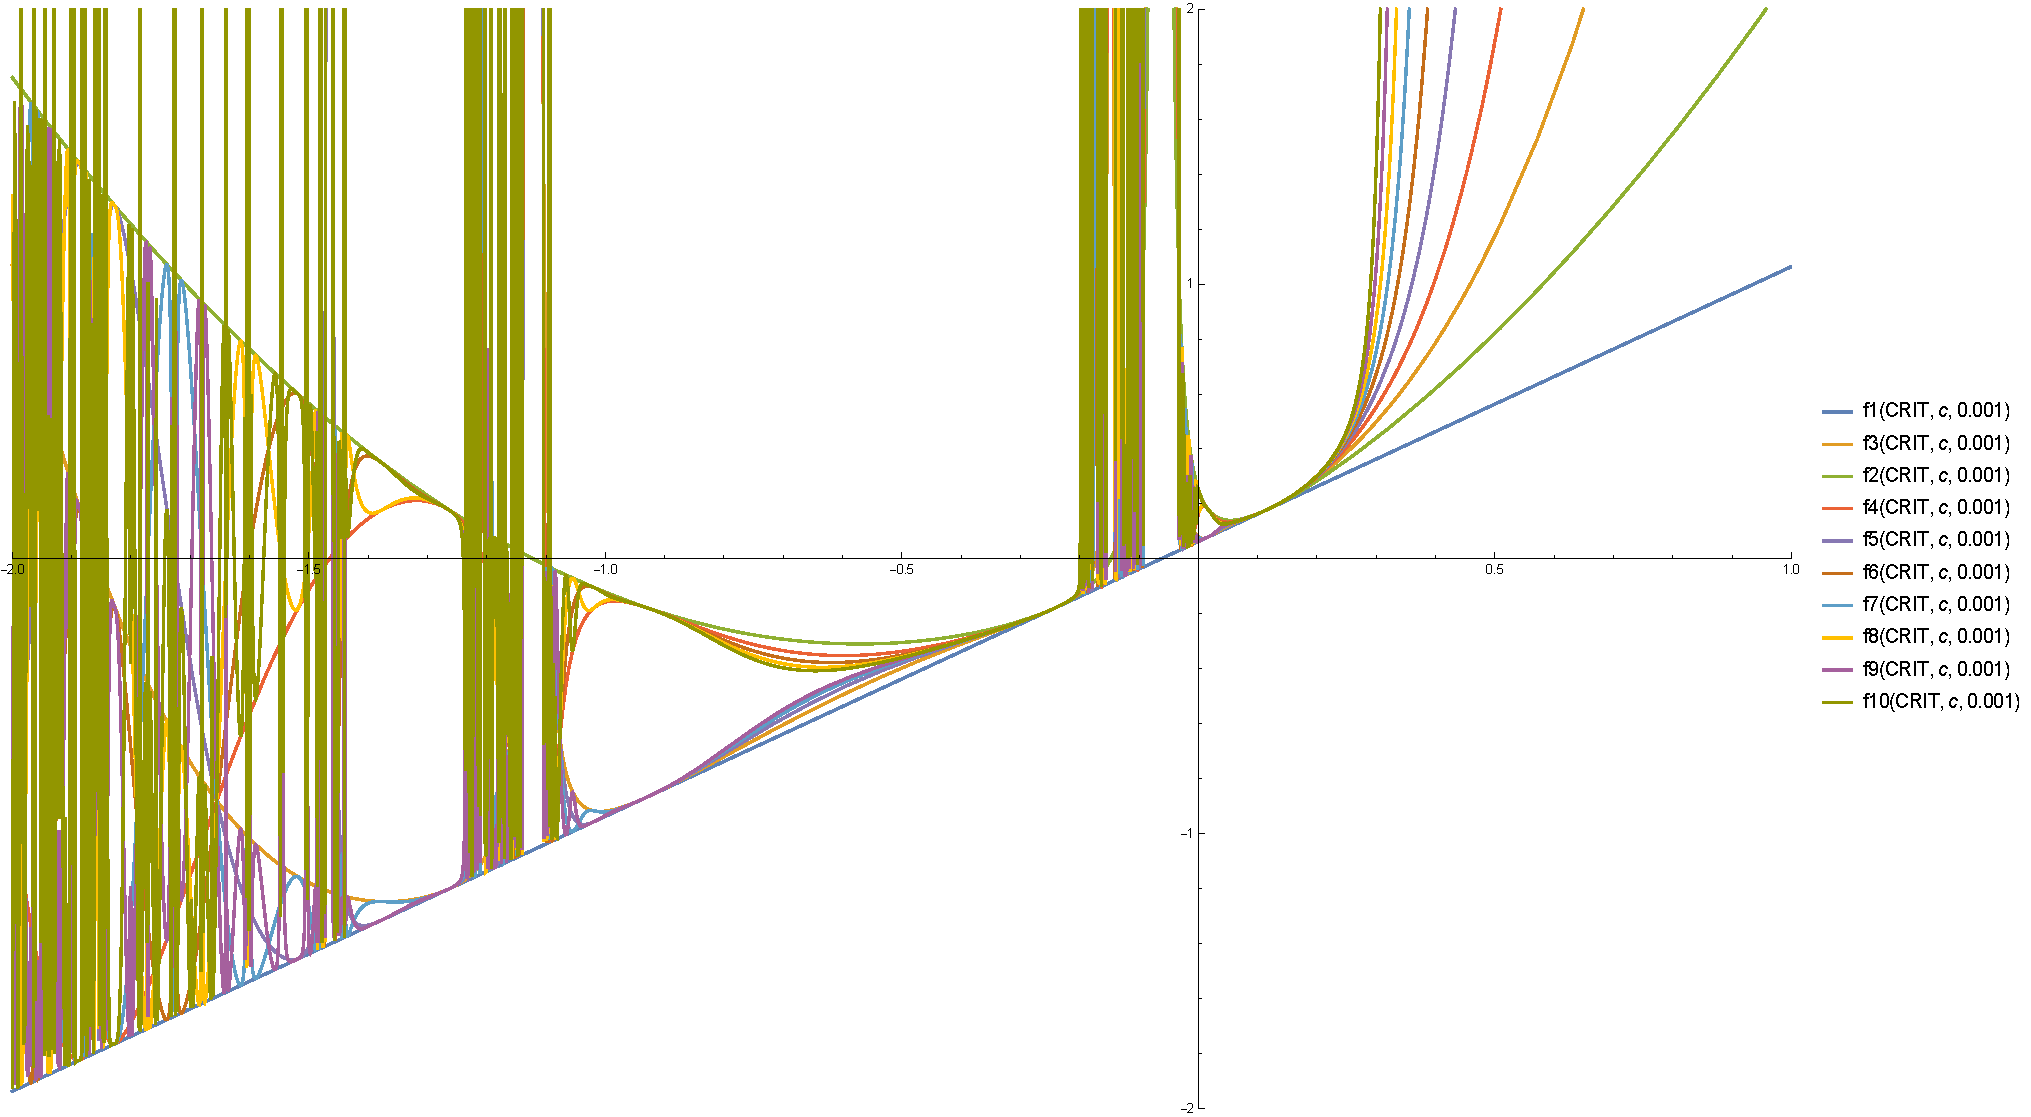
\includegraphics[width=\textwidth]{./img/pert}
					\caption{Orbit diagram of $x^2 + c + \frac{.001}{x^2}$}
					\label{pert}
			\end{subfigure}%
			\begin{subfigure}[b]{0.5\textwidth}
					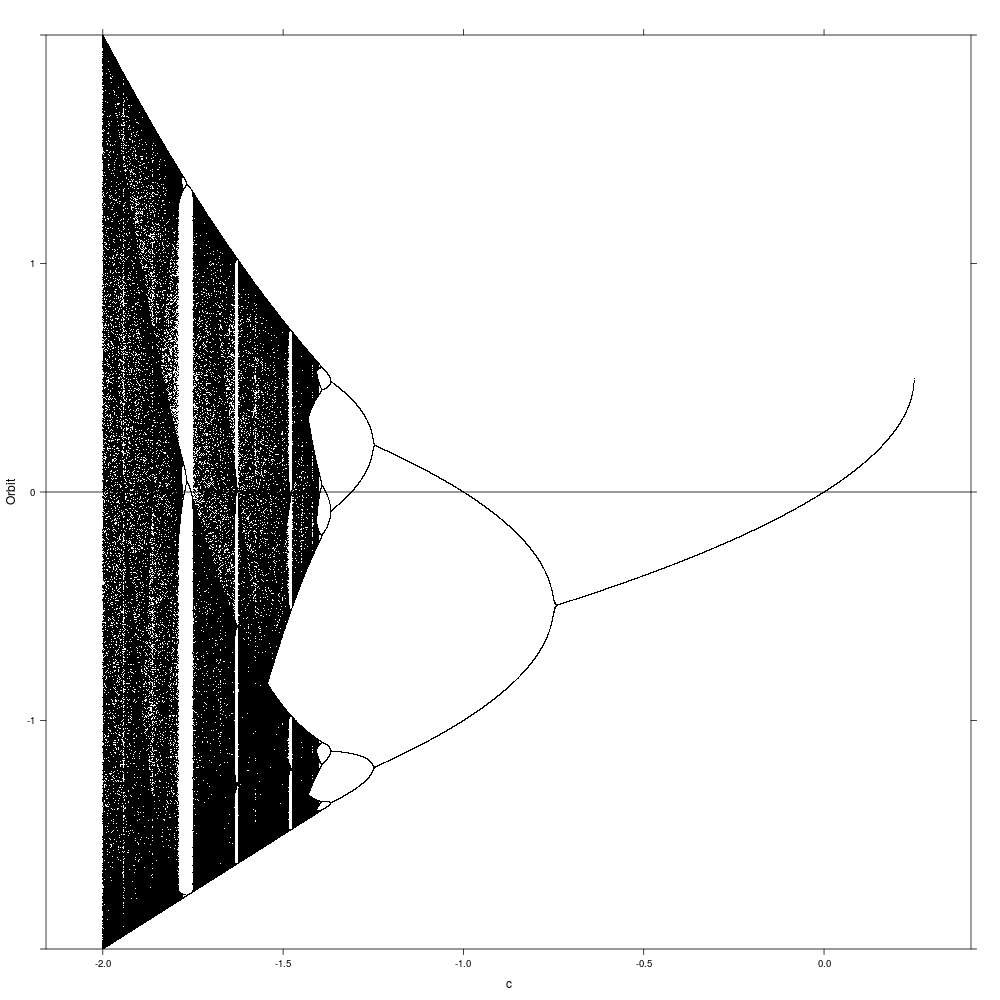
\includegraphics[width=\textwidth]{./img/orig}
					\caption{Orbit diagram of $x^2 + c$}
					\label{stand}%
			\end{subfigure}
			\caption{Orbit diagrams of the perturbed system and the original system}\label{fig:orbits}
		\end{figure}

		Now that we have established that the behavior of the critical orbit helps determine the behavior of the system, we can perform a few numerical experiments to discover where the dynamics of the perturbed system varies from the dynamics of the original quadratic map $Q_c (x) = x^2 + c$. As previously discussed, a standard analysis of the behavior of the critical orbit is to create an orbit diagram as shown in Figure \ref{pert} and Figure \ref{stand}. Immediately we can see some major differences between the behavior of the two families. One of the most notable differences is on the parameter interval $c\in (-.25, .05)$ (magnifications of which are shown in Figures \ref{pertz2} and \ref{pertz1}).

		The following section will discuss the behavior of the system for $c$ intervals which are either straightforward or analogous to the behavior of the original quadratic map. Subsequent sections will then describe some of the behavior where the perturbed  map acts quite differently than the standard map, providing some instances of interesting critical orbit behavior. Since $\beta = .001$ is fixed from this point forward, we will refer to $f_{c, \beta = .001}$ as $f_{c}$.

		\begin{figure}[h]
			\centering
			\begin{subfigure}[b]{0.5\textwidth}
					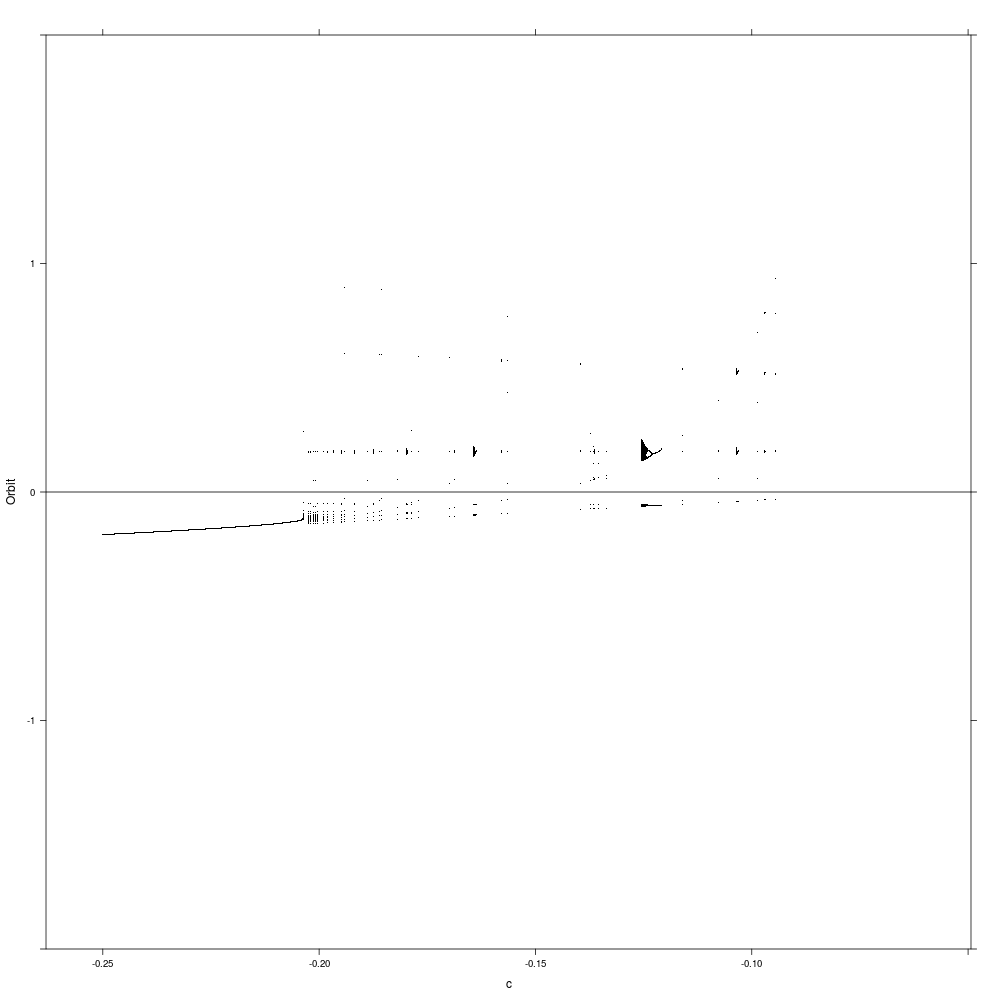
\includegraphics[width=\textwidth]{./img/pertzoom2}
					\caption{$c\in (-.25, -.062456)$}
					\label{pertz2}
			\end{subfigure}%
			\begin{subfigure}[b]{0.5\textwidth}
					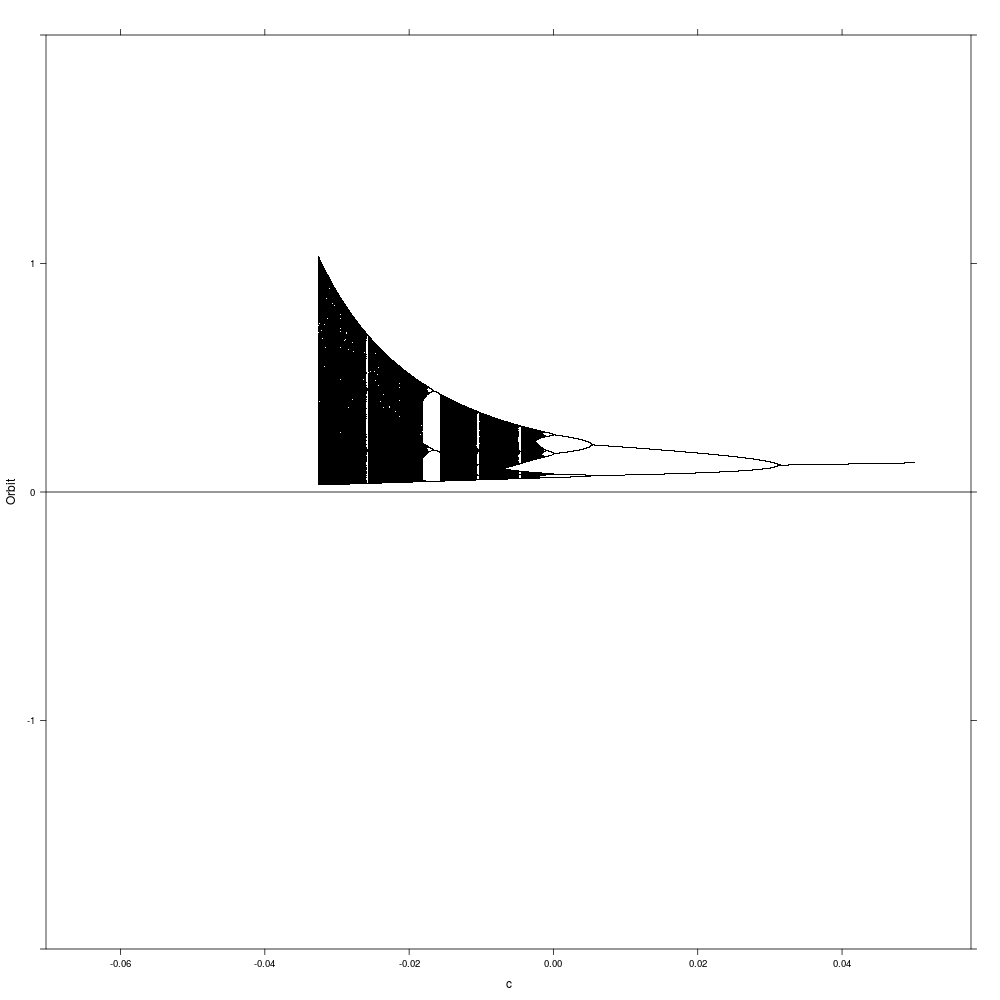
\includegraphics[width=\textwidth]{./img/pertzoom1}
					\caption{$c\in (-.062456, .05)$}
					\label{pertz1}%
			\end{subfigure}
			\caption{Zooms of the perturbed system's orbit diagram}\label{fig:orbits2}
		\end{figure}